\section{Background}\label{sec:background}

TODO introduction
\subsection{Spark}\label{subsec:spark}
Spark is the probably most widely used and industry accepted cluster computing model.
It improves over former computing models, e.g. MapReduce~\cite{mapreduce}, Hadoop~\cite{hadoop} or Haloop~\cite{haloop},
by allowing to cache results in memory between multiple queries, using so-called resilient
distributed datasets~\cite{rdd}; often abbreviated to RDD.

This section introduces Spark and is organized in four subsections.
\Cref{subsubsec:resilient-distributed-datasets} describes the core data structure of Spark: the RDD's.
In~\cref{subsubsec:spark-architecture}, we explain the different components and processes in a Spark cluster.
The query optimizer of Spark, Catalyst, is explained in~\cref{subsubsec:catalyst}.
It is the component we integrate our \textsc{WCOJ} with;
therefore, it is the module of Spark that is most relevant to this thesis.
Finally, in~\cref{subsubsec:broadcast-variables} we highlight important details about \textit{Broadcast variables} which are used
to implement our parallel worst-case optimal join.

\subsubsection{Resilient distributed datasets} \label{subsubsec:resilient-distributed-datasets}
RDD's form the core of Spark.
However, for this thesis, it is not necessary to understand them in great detail.
In the next paragraph, we give a short introduction to the relevant aspects of RDD's.
For the interested reader, a more in-depth description is given in the original paper~\cite{rdd}.

Resilient distributed datasets describe a distributed collection of data items of a single type.
In contrast, to other distributed share memory solutions, RDD's do not use fine-grained
operations to manipulate single data items but coarse-grained operations which are applied
to all data items, e.g. \textit{map} to apply a function to each data item.
These operations are called \textit{transformations}.
An RDD is built starting from a persistent data source and multiple transformations to
apply to this data source.
One can store the transformations applied to the input data source as a directed acyclic graph, the so-called \textit{lineage graph}.
This graph fully describes the dataset without materializing it because the transformations are deterministic.
Hence, the dataset can be computed and recomputed on demand, e.g. when the user asks for the count
of all items in the set.
Operations which require that the data in the RDD is computed are called \textit{actions}.

RDD's are distributed by organizing their data items into partitions.
The partitioning can be chosen by the user or the Spark query optimizer such that it allows to run transformations on all partitions
in parallel.
For example, one might choose a round-robin partitioning to generate splits of equal size when reading data items from disk or one
groups items by hashing a specific key to support parallelizable aggregation on that key per partition.
The process of repartitioning an RDD is called a \textit{shuffle}.
It is an expensive operation because it involves writing and reading the whole RDD to disk.

Describing datasets as RDD's comes with two main benefits.
First, it is resilient because if the dataset or some partitions of it get lost, it is possible to recompute them from persistent storage
using lineage graph information.
Second, it allows Spark to compute RDD's in parallel.

Spark can parallelize the computation of RDD in two ways.
First, by data-parallelism, since different partitions of an RDD can
be computed independently from each other.
Second, by task parallelism, because some parts of the DAG can be computed without dependence of the others.
Indeed, it is possible to compute all parts of an RDD in parallel which are not related in a topological sort of the graph.

\subsubsection{Spark architecture} \label{subsubsec:spark-architecture}
Spark allows the user to run his program on a single machine or hundreds of machines organized in a cluster.
In this section, we explain the architecture that allows this flexibility.
\Cref{fig:spark-cluster} shows the schematics of a Spark cluster setup.

\begin{figure}
    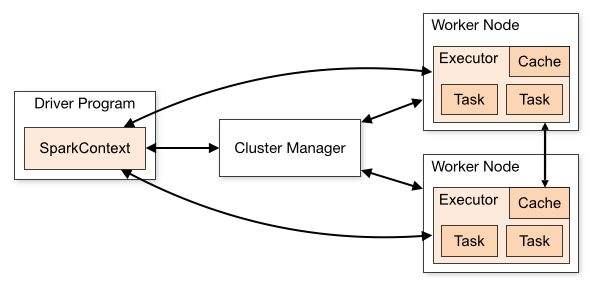
\includegraphics[width=\textwidth]{figures/spark-cluster.png}
    \caption{
      Schematics of a Spark cluster with two workers, each of them with one exectuor and two threads per executor.
      Source: Apache Spark Documentation, https://spark.apache.org/docs/latest/cluster-overview.html
    }
    \label{fig:spark-cluster}
\end{figure}

In Spark, each physical machine is called a \textit{worker}.
On each worker, Spark starts one or multiple Spark processes in their own JVM instance; each of them is called \textit{executor}.
Nowadays, many Spark deployments use a single executor per worker\footnote{This is the setup Databricks uses; Databricks is the leading
maintainer of the Spark platform and offers professional deployment to many customers.}.
Each executor runs multiple threads (often one per core on its worker) to execute multiple tasks in parallel.
In total, a Spark cluster can run \textit{\# workers} $\times$ \textit{\# executors per worker} $\times$ \textit{\# threads per executor} tasks
in parallel.

Spark uses two kinds of processes to execute an application: a \textit{driver program} and multiple \textit{executors}.
When started, the driver program acquires resources from the \textit{cluster manager} for its executor processes.
These executors stay alive during the whole Spark application.
Then, the driver program continues executing the Spark application.
When it encounters parallelizable tasks, it schedules them on the available executors.

All tasks scheduled on the same executor share a cache for in-memory data structures like \textit{Broadcast variables} or persisted RDD
partitions.
This is important in the context of this thesis because it means that we cache the input graph once per executor;
which in many Spark deployments is once per worker or physical machine.
This would not be possible if different tasks in the same JVM would not share the same cache.

Spark allows the user to choose a cluster manager to manage resources in the cluster.
It comes with good integration for Hadoop YARN~\cite{yarn}, Apache Mesos~\cite{mesos} and Kubernetes~\cite{kubernetes}, as well as,
a standalone mode where Spark provides its own cluster manager functionality.
Finally, one can run Spark on a single machine in \textit{local mode}.
In local mode, the driver program and a single executor share a single JVM.
The executor uses the cores assigned to Spark to run multiple worker threads.
For our experiments, we run Spark purely in local mode.

\subsubsection{Catalyst} \label{subsubsec:catalyst}
Catalyst~\cite{spark-sql} is Spark's query optimizer.
It can process queries given as a SQL string or described using the DataFrame API.
From a given query it constructs an executable \textit{physical plan}.
The query compilation process is organized in multiple stages.
Its inputs and stages are shown in~\cref{fig:catalyst-stages}.
Below we explain these in order.
We use the triangle given by the datalog rule $COUNT(triangle(A, B, C)) \leftarrow R(A, B), S(B, C), T(A, C), A < B < C $ as
a running example.

\begin{figure}
    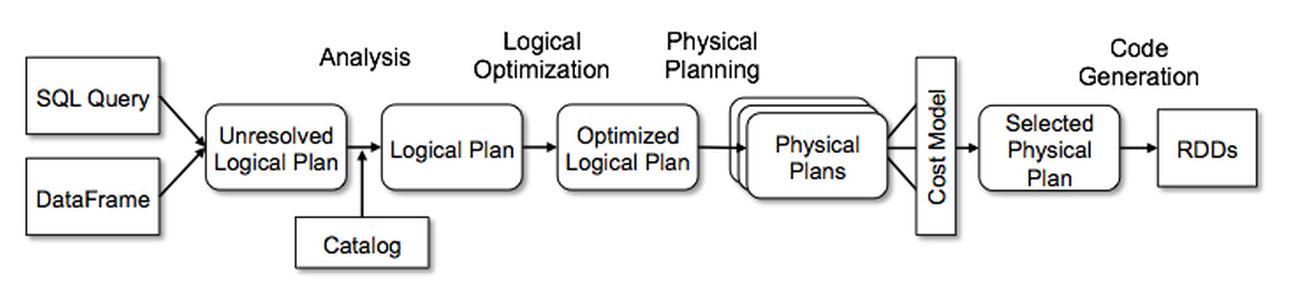
\includegraphics[width=\textwidth]{figures/catalyst-stages.png}
    \caption{
    Input and stages of the Catalyst optimizer.
    Source: Databricks Blog, https://databricks.com/blog/2015/04/13/deep-dive-into-spark-sqls-catalyst-optimizer.html
    }
    \label{fig:catalyst-stages}
\end{figure}

The input of Catalyst is a query in the form of a DataFrame or SQL string.
From this the optimizer builds a \textit{unresolved logical plan}.
This plan can include unresolved attributes, e.g. attribute names which are not matched to a specific
data source yet or which have no known type.
To resolve this attributes Catalyst uses a \textit{Catalog} of possible bindings which describe the
available data sources.
This phase is referred to as \textit{Analysis} and results in a \textit{logical plan}.
The logical plan represents \textit{what} should be done for the query but not exactly \textit{how},
e.g. it might contain a Join operator but not a Sort-merge join.

We show the logical plan for the triangle query in~\cref{fig:triangle-logical-plan}.
As we see, the query is represented as tree where the vertices are operators and the edge indicate dataflow from
one operator to another.
The leaves of the tree are three aliases of the edge relationship.
Two of these source relationships are the input the join between \textit{R} and \textit{S} via \textit{B}.
The result of this join and the leaf relationship \textit{T} are input to the second join.
The tuples produced by this join are filtered to fulfil $A < B < C$.
Finally, at the root of the tree, there is an aggregation to count all results and report the sum.

\begin{figure}
    \centering
    \subfloat[Logical plan\label{fig:triangle-logical-plan}]{\includesvg[width=0.4\textwidth]{triangle-logical-plan}}
    \subfloat[Physical Plan\label{fig:triangle-physical-plan}]{\includesvg[width=0.6\textwidth]{triangle-physical-plan}}
    \caption{Logical and physical plan for the triangle count query as generated by Catalyst.}
\end{figure}

The \textit{logical optimization phase} applies batches of rewriting rules until a fixpoint is reached.
A simple example of a logical optimization would be rewriting $2 + 2$ into $4$.
In the running example of the triangle query, this phase pushes the filters into the two joins.
This optimization is called Filter Pushdown.
It is efficient because it applies filters earlier within the pipeline reducing the number tuples to process by later operators.

From the \textit{optimized logical plan} the optimizer generates one or multiple \textit{physical plans} by
applying so called \textit{Strategies}.
They translate a logical operator in one or multiple \textit{physical operators}.
\textit{Strategies} are also allowed to return multiple physical plans for a single \textit{logical plan}.
In this case, the optimizer selects the best one according to a \textit{cost model}.

The physical plan for the triangle query is shown in~\cref{fig:triangle-physical-plan}.
We see multiple examples of translation of a logical operator, which describes what to do, to its physical pendant that also
describes how to do it: the \textit{TableScan} becomes a \textit{CSVRead} and the \textit{Joins} are implemented as
\textit{BroadcastHashJoins}.

Furthermore, we see the introduction of exchanges.
\textit{BroadcastExchanges} precede the \textit{BroadcastHashJoins}.
They build a hashtable from their input operators and make them available as a broadcast variable to all executors of the cluster;
we explain broadcast variables in depth in~\cref{subsubsec:broadcast-variables}.
When an executor is tasked to execute the hash join operator, it acquires the broadcasted hashtable and executes a local hash join
of its assigned partitions.

Another exchange operator is introduced for the aggregation.
It is broken up into a partial aggregation directly after the last join, an exchange reorganizing all partial counts into a single
partition and a second aggregation over that partition to calculate the total count.
The last is a good example of Catalyst introducing a shuffle.

To conclude, the translation to a physical plan translates logical operators into concrete implementations of these and adds exchanges
to organize the data such that it can be processed independently in partitions.

After generating and choosing a physical plan, Catalyst enters the \textit{code generation} phase in which it compiles Java byte code for
some of the physical operators.
This code executes often magnitudes faster than interpreted versions of the same operator~\cite{spark-sql} because
it can be specialized towards this particular query, e.g. if a join operates only on integers, code
generation can prune all code paths dealing with strings.
Indeed, the code generation phase is part of another Spark project called
\textit{Tungsten}~\cite{tungsten-project,tungsten-code-generation}.
In this thesis, we do not build any code generated physical operators.
Hence, we do not treat this topic in depth.
It is enough to know that all freshly generated Java code is wrapped into a single physical operator.
Therefore, it integrates seamlessly with interpreted operators.

Finally, Catalyst arrives at an optimized physical plan which implements the query.
The execution of this plan is called
\textit{structured query execution}~\cite{spark-internals-structured-query-execution}.
It translates the plan into RDD operations implemented by Spark's core.
Hence, the result of Catalysts query compilation is an RDD representing the query.
One should note that structured query execution does not materialize the query: the result is an RDD which is a none
materialized representation of the operations necessary to generate the result.
In this thesis, we are not concerned with the internals of RDD's.
We do not need to introduce any new RDD operations or even touch Spark's core functionality.
Thanks to the extensibility of Catalyst, we can integrate worst-case optimal joins by adding one logical operator, multiple
physical operators and a Strategy to translate between them.

\subsubsection{Broadcast variables} \label{subsubsec:broadcast-variables}
\textit{Broadcast variables} readonly variables which are accessible by all tasks.
They are initialized once by the driver program and should not be changed after initialization.
The process of broadcasting them is handled by Spark.
It is guaranteed that each broadcast variable is sent only once to each executor and allows it to be spilled to disk if it is not
possible to keep the whole value in memory.
Furthermore, `Spark attempts to distribute broadcast variables using efficient broadcast algorithms to reduce communication
costs'~\cite{rdd-programming-guide}; currently Spark uses a BitTorrent-like communication protocol\footnote{See Spark sources:
\texttt{org.apache.spark.broadcast.TorrentBroadcast}}.
Once sent, they are cached once per executor~(see also~\cref{subsubsec:spark-architecture}) and shared by all tasks on this executor.
They are cached in deserialized form in memory but can be spilled to disk if they are too big.
In this thesis, we use broadcast variables to cache the edge relationship of the graph on all workers.

\subsection{Graph pattern matching}
% Definition of graph pattern matching
% Important queries can be covered by full, conjugutive E1 formulaes
%  or equijoins
%

\subsection{Worst-case optimal join algorithm}\label{subsec:worst-case-optimal-join-algorithm}
The development of worst-case optimal joins started in 2008 with the discovery that the output size of a relational query
is bound by the fractional edge number of its underlying hypergraph~\cite{agm}.
In short, this bound proves that traditional, binary join plans perform asymtopically worse than theoretical possible
for the worst-case database instances, e.g. heavely skewed instances.
For instance, the worst-case of the triangle query is in $\mathcal{O} (N^2)$ , while the AGM bound
shows the possibility to solve it in $\mathcal{O} (N^{3/2})$.
The AGM bound has been treated widely in literature~\cite{skew-strikes-back,andreas,agm}.
A particular good explanation is given by Hung Ngo et al in~\cite{skew-strikes-back}.
We refer the reader to these papers for further information.
In the next paragraph, we discus different algorithms matching the AGM bound which are called worst-case optimal joins.

In 2012, Ngo, Porat, Re and Rudra published a join algorithm matching this bound~\cite{nprr}, called \textit{NPRR} join.
In the same year, Veldhuizen proved that the algorithm \textit{Leapfrog Triejoin} used in LogicBlox,
a database system developed by his company, is also worst-case optimal with regards to the fractional edge number bound.
We often abbreviate Leapfrog Triejoin to \textsc{LFJT}.
Both algorithms have been shown to be instances of a single algorithm, the \textit{Generic Join}, in 2013 Ngo et al.~\cite{skew-strikes-back}.

We identified three worst-case optimal join algorithm: NPRR, LFTJ and Generic Join.
We choose Leapfrog Triejoin as the basis for our work.
The argumentation for this decision is given below.
First, we identify the main criteria this choice.
Then, we use them to compare the different algorithms.

The most important argument for our decision is the degree to which the algorithm has been shown
to be of practical use.
In particular, the number of systems it is used in and openly available data on its performance.
If an algorithm is used in academia as well as in industry, we deem this as a big advantage.
This criteria carries a lot of weight because the first literature on worst-case optimal joins
has been rather theoretical but in our work we take a more praxis and system oriented perspective.

The practical character of our work also motivates the second dimension we compare the algorithms in, namely
ease of implemenation.
If two of the three algoritms both have well proven performance, we would like to choose the algorithm
that takes less time to implement and is easier to adapt and experiment with.
That is to be able to spent more time on evaluation and optimizations for the graph use-case, instead of,
time spent on replicating existing work.

The Leapfrog Triejoin is used in two commercial database solutions:
LogicBlox~\cite{logicBlox} and RelationalAI~\footnote{https://www.relational.ai/}.
Its performance has been reported on in two publications~\cite{myria-detailed,olddog}.
In particular, it beats various general and graph specific databases for graph pattern matching~\cite{oldgo}, i.e.
PostgresSQL, MonetDB, NEO4J, graphLab and Virtuoso.
The broadest study of its performance uses 15 different datasets and 7 queries~\cite{olddog}.
We conclude that the performance of \textsc{LFTJ} is well established by peer reviewed publications
as well as industrial usage.
% TODO find cites for graphlab and Virtuoso

\textit{NPRR} has been well analyzed from the theoretical point of view.
However, we are not able to find any openenly available sources with performance measurements.
This disqualifies \textsc{NPRR} as basis for our thesis.

\textit{Generic Join} is used in at least three academic graph processing engines,
namely GraphFlow~\cite{graphflow}, EmptyHeaded~\cite{emptyheaded} and a unnamed implemenation in
Timely DataFlow~\cite{ammar2018distributed}.
All three show good performance.
However, we are not aware of any commercial systems using \textsc{GJ}.

The comparision of Leapfrog Triejoin, \textsc{NPRR} and \textit{Generic Join} by proven performance
rules out \textsc{NPRR} and puts \textsc{LFTJ} and \textsc{GJ} on a similar level.
Next, we compare these two algorithm in ease of implementation.

The description of the Leapfrog Triejoin implementation in its original paper~\cite{lftj} is excellent.
Furthermore, multiple open source implementation exists~\cite{de-witt,myria-detailed}.
In particular, the implementation of Christian Schroeder for a course at Oxford is helpful because it is standalone and
does not require us to understand a whole system\footnote{TODO GitHub Dewitt}.

\textit{Generic Join} is described as a generalization of \textsc{NPRR} and Leapfrog Triejoin in its original
paper~\cite{skew-strikes-back}.
Although, well written and algorithmically clear, this explanation is much less practical than the one given for \textsc{LFTJ} which
is backed by a executable implementation.

To conclude, we choose Leapfrog Triejoin as basis for our work based on its openely available records of performance, use in
academic as well as industrial systems and good description for direct implementation.
Furthermore, Peter Boncz (supervisor of this thesis) has direct contact to the inventors of \textsc{LFTJ} giving us access to valuable
expertise if necessary.

\subsubsection{LeapfrogTriejoin}



% Use in industry
The Leapfrog Triejoin gives strong theoretical guarantues which have been proven to be worst-case optimal in~\cite{lftj}.
Moreover, the \textsc{LFTJ} has been shown to be of practical use in multiple systems and papers.
It is at the core of the commercial LogicBlox database system~\cite{lftj} and in the products of
RelationalAI\footnote{https://www.relational.ai/}, the latter company of its inventors.
Hence, showing its worth in industry.
In academia, Leapfrog Triejoin has been shown to beat traditional binary join plans employing Hashjoins or Sort-Merge joins,

% full, conjugative query == equi joins?
%  equi joins important for graph pattern matching
%  concentrate on only that

% LFTJ paper proof concentrates on full, conjugative queries and extends it to existence1 queries, this
% is first order logic without all quantifier and no negated existence

The Leapfrog Triejoin is a variable-oriented join.
Given an input queries, it requires a variable ordering.
For example in the triangle query $triangles(a, b, c) \leftarrow R(a, b), S(b, c), T(a, c)$,
the variable ordering could be $a, b, c$.
Furthermore, the Leapfrog Triejoin requires that its input relationships to be sorted by lexicographic, ascending order over the given
variable ordering.
Then it fixes one possible binding for $a$, one for $b$ given $a$ and finally one for $c$ given $a$ and $b$.
This allows it to enumerate the result of the join query without intermediary results.
The process can be thought of as a backtracking, depth-first search for possible bindings.

% TODO figures of layered LFTJ
The algorithm to implement this search uses three components which are composed in a layered fashion.
The concrete composition used for the triangle query is shown in~\cref{fig:lftj-layers}.
In this figure, we see three layers each of them made of one or more instances of a component.
The components are the \textit{TrieIterator}, \textit{LeapfrogJoin} and \textit{LeapFrogTriejoin}.
In the next paragraphs, we explain each layer in order starting with the lowest layer.

The lowest layer is made of one \textit{TrieIterator} per input relationship.
In our example, we have three instances one for R, S and T each.
The \textit{TrieIterator} interface represents the input relationship as a trie with all values for
the first attribute on the first level, the values for the second attribute on the second level and so
on; an example for this is shown in~\cref{fig:trie-example}.

The trie contains one level per attribute of the relationship;
in this case, this are two levels one for $a$ and one for $b$.
Each level is made of all possible values for this attribute.
All tuples of the relationship can be enumerated by a depth-first traversal of this trie.

The \textit{TrieIterator} component offers five methods shown in~\cref{table:trieIterator-inteface}.
The \textit{open} and \textit{up} methods control the trie level the iterator is positioned at;
\textit{open} moves it one level down and \textit{up} moves it one level up.
Additionally, \textit{open} places the iterator at the first value for the next level and the up
method returns to the value of the upper level that was current when the next level was opened.
We call these two methods the vertical component of the \textit{TrieIterator} interface.

The other four methods are called linear component.
All of them operate on the current level of the \textit{TrieIterator}.
The \textit{key} function returns the current key.
The \textit{next} method moves the iterator to the next key on the same level.
The \textit{seek(key)} operation finds the least upper bound for its parameter \textit{key}.
Finally, the \textit{atEnd} method returns \textit{true} when the iterator is placed behind the last value of the current level.


The middle layer is build of one \textit{LeapfrogJoin} per variable in the join.
This join generates possible bindings for its variable by intersecting the possible values for all input relationship containing the
variable.
Therefore, it operates on the linear component of all \textit{TrieIterators} of relationships with this variable.
\Cref{fig:lftj-layers} for the triangle query shows three \textit{LeapfrogJoin} instances (for $a, b$ and $c$);
each of them uses two \textit{TrieIterators}.

The \textit{LeapfrogJoin} interface has five methods shown in~\cref{table:leapfrogJoin-interface} with their required asymptopical performance.
In the following paragraphs, we explain each of them.
In short, the join offers a iterator interface over the intersection of its input iterators.
This intersection is found by repeatingly seeking the value of the largest input iterator in the smallest input iterator.
This process resemples a frog taking a leap which gives the join its name.
When all iterators point to the same value leapfrogging stops and the value is emitted as part of the intersection.

The \textit{init} operation sorts the input iterator by their current key and finds the first value of the intersection.
To find the first value it uses the private method \textit{leapfrogSearch} which is the work-horse of the whole join.
The algorithm of this method is shown in~\cref{alg:leapfrogSearch}.
This method loops the process of calling the \textit{seek} method of the its smallest input iterator with the key of the largest input
iterator until the smallest and the largest (and therefore all iterators) point to the same value.

\begin{algorithm}[H]
    \KwData{
      iters \# sorted array of TrieIterators \;
      p  \# index of the smallest iterator\;
    }
   \KwResult{Either atEnd is true or key is set to next key of intersection}
    maxKey $\leftarrow$ iters[p \% iters.length].key()\;
   \While{iters[p].key() $\neq$ maxKey}{
     iters[p].seek(maxKey)\;
     \eIf{iters[p].atEnd()} {
       atEnd $\leftarrow$ true\;
       return\;
     } {
       maxKey $\leftarrow$ iters[p].key()\;
       p $\leftarrow$ (p + 1) \% k\;
     }
   }
   key $\leftarrow$ iters[p].key()
   \caption{leapfrogSearch()}
   \label{alg:leapfrogSearch}
\end{algorithm}
% TODO styling

The \textit{leapfrogNext} method moves the join to its next value.
Internally, it uses the \textit{next} function of its smallest iterator and then \textit{leapfrogSearch}.

The operation \textit{leapFrogSeek(key)} first uses the \textit{seek} method of the smallest input iterator to forward it to \textit{key};
then it uses \textit{leapfrogSearch} to either verify that this key is available in all iterators (hence in the intersection) or
to find the upper bound of this key.

Finally, the functions \textit{key} and \textit{atEnd} return the current key or if the intersection is complete respectively.

The last layer is a single \textit{LeapfrogTriejoin} instance.
It interacts with both lower layers to enumerate all possible bindings for the join.
For this it aquires one binding for the first variable from the corresponding \textit{LeapfrogJoin}.
Then it moves the \textit{TrieIterators} containing this variable to the next level and
finds a binding for the second variable using the next \textit{LeapfrogJoin}.
This process continues until all variables are bound and a tuple representing this binding is emitted
by the join operator.
Then it finds the next possible binding by backtracking.

The algorithm used for the backtracking depth-first traversal is shown in~\cref{alg:leapfrogTrieJoin-state-machine}.
This traversal needs to stop each time when a complete tuple has been found to support the iterator interface of the join.
Therefore, it is implemented as a state-machine which stops each time the deepest level is reached and all variables are bound
(loop condition in line 35). % LINE
The next action of the state machine is determined by the outcome of the current action.
Hence, we can characterize the state machine by describing each possible action and its possible outcomes.
There are three possible actions: \textit{next}, \textit{down} and \textit{up}.
We summarize the possible actions, conditions for the next action and if the main loop of the state machine yields the next tuple
in~\cref{table:lftj-state-machine} and describe each action below.

\begin{algorithm}[H]
    \kwData{
      depth \\* the index of the variable to find a binding for, range from -1 to #variables - 1 *\\ \;
      MAX_DEPTH \\* the number of variables \\*
      bindings \\* array holding the current variable bindings or $-1$ for no binding \\* \;
      action   \\* state of the state machine \\* \;
    }
    \Repeat{!((depth == MAX\_DEPTH \&\& bindings[MAX\_DEPTH] $\neq$ -1)) || atEnd} {
      \Switch{action} {
        \Case{NEXT} {
            leapfrogJoins[depth].leapfrogNext() \;
            \eIf{leapfrogJoins[depth].atEnd()} {
                action $\leftarrow$ UP \;
            } {
                bindings(depth) $\leftarrow$ leapfrogJoins[depth].key() \;
                \If{depth == MAX\_DEPTH} {
                    action $\leftarrow$ NEXT
                } {
                    action $\leftarrow$ DOWN
                }
            }
        }
       \Case{DOWN} {
          depth $\leftarrow$ depth + 1 \;
          trieJoinOpen() \;
          \eIf{leapfrogJoins[depth].atEnd()} {
            action $\leftarrow$ UP \;
          } {
            bindings(depth) $\leftarrow$ leapfrogJoins[depth].key() \;
          \eIf{depth == MAX\_DEPTH} {
             action $\leftarrow$ NEXT
          } {
            action $\leftarrow$ DOWN
          }
          }
       }
        \Case{UP} {
          \eIf{(depth == 0)} {
            atEnd $\leftarrow$ true \;
          } {
            depth $\leftarrow$ depth - 1 \;
            trieJoinUp() \;
            \eIf{leapfrogJoins[depth].atEnd()} {
                action $\leftarrow$ UP \;
            } {
                action $\leftarrow$ NEXT \;
            }    
          }
        }
      }
    }  
    \caption{LeapfrogTrieJoin state machine}
    \label{leapfrogTrieJoin-state-machine}
    % TODO mention triejoinopen and triejoinUP
\end{algorithm}
% TODO styling
The \textit{next} action moves the \textit{LeapfrogJoin} at the current depth to the next possible binding for its variable (line 2). % LINE
If the \textit{LeapfrogJoin} reached its end, we continue with the \textit{up} action (line 4), % LINE
otherwise we set the binding and continue by another \textit{next} action, if we are at the deepest level or by moving
to the next deeper level by the \textit{down} action (line 7). % LINE

The \textit{down} action moves to the next variable in the global variable ordering by opening all related \textit{TrieIterators}
and initializing the corresponding \textit{LeapfrogJoin} (line 20 call to \textit{trieJoinOpen}) % LINE.
A \textit{down} can be followed by an \textit{up} if the \textit{LeapfrogJoin} is \textit{atEnd} (line 22),
by a \textit{next} action if the trie join is at its lowest level (line 25), or by another \textit{down} action to reach the deepest level.

The \textit{up} action can signal the completion of the join if all bindings for the first variable in the global ordering have
been explored, or in other words, the first \textit{LeapfrogJoin} is \textit{atEnd} (condition
\textit{depth == 0 $\wedge$ action ==  UP} line 28). % LINE
Otherwise, all \textit{TrieIterators} corresponding to the current variable are moved upwards by calling \textit{triejoinUp} (line 31)
which also updates \textit{depth} and \textit{bindings}.  % LINE
Then, this action is followed by another \textit{up} or a \textit{next} depending on \textit{atEnd} of the current \textit{LeapfrogJoin}
(lines 32). % LINE

\begin{table}[]
    \centering
    \begin{tabular}{@{}llll@{}}
        \toprule
        Action                & Condition                                  & Next action & Yields \\ \midrule
        \multirow{3}{*}{NEXT} & \textit{lf.atEnd}                                   & UP          & no     \\
        & \textit{$\neg$lf.atEnd} $\wedge$ \textit{reachedMaxDepth}             & NEXT        & yes    \\
        & \textit{$\neg$lf.atEnd} $\wedge$ \textit{$\neg$reachedMaxDepth}            & DOWN        & no     \\
        & & &\\
        \multirow{3}{*}{DOWN} & \textit{lf.atEnd}                                   & UP          & no     \\
        & \textit{$\neg$lf.atEnd} $\wedge$ \textit{reachedMaxDepth}             & NEXT        & yes    \\
        & \textit{$\neg$lf.atEnd} $\wedge$ \textit{$\neg$reachedMaxDepth}            & DOWN        & no     \\
        & & &\\
        \multirow{3}{*}{UP}     & \textit{depth = 0}, means highest \textit{lf.atEnd} is true & -- (done)         & yes    \\
        & \textit{lf.atEnd}                                   & UP          & no     \\
        & \textit{$\neg$lf.atEnd}                                  & NEXT        & no     \\ \bottomrule
    \end{tabular}
    \caption{Summary of actions, conditions for the following action and if a complete tuple has been found.
    \textit{reachedMaxDepth} is true if we currently find bindings for the last variable in the global order.
    \textit{lf} abbreviates the \textit{LeapfrogJoin} of the current variable.
    The columns \textit{Yields} details if the main loop of the state machine yields before computing the next action,
    this is the case, when all variables have been bound.
    }
    \label{table:lftj-state-machine}
\end{table}


%    different backing datastructures B-Trees, Arrays Tributary join.
%       in this work we add CSR

% Inputs:
%      attributes subsequent of the join variable ordering
% variable ordering needs to be discussed before
%    only existence or the whole problem of join variable ordering?



% Queries: olddog, Semih's paper,
%    Mostly for graphs

% background over "typical" graph pattern matching queries needed
%   olddog good introduction about binary joins vs wcoj for graph pattern matching
% background about graph pattern matching needed

% background on binary join operators?
% comparision, intermediate results
%  intuitive understanding of why better?

% WCOJ against graph engines (oldog)
% Comparision with other systems: oldog, graphlab, virtuoso, monetdb, pssql, neo4j


% TODO find placement
\paragraph{Extentsions}
The algorithm described below and all variants implemented in this thesis can process joins of the full conjunctive fragment of first
order logic or conjugative equi-joins in relational algebra terms.
Possible extentsions to disjunctions, ranges (none-equi joins), negation, projection, functions and scalar operations on join variables are
described in the original Leapfrog Triejoin paper~\cite{lftj}.
However, they are not relevant to the core of this work because many interesting graph patterns can be answered using the full conjunctive
fragment, e.g. cliques or cycles.

% Codegeneration studied by RelationalAi
% Compression studied by Richard
\paragraph{Variable ordering}  % TODO move all sections one up and use of chapter?
Finding a good variable ordering for the \textsc{LFTJ} is an interesting research problem in itself.
We are aware of two existing approaches.

The first is to create and maintain representative samples for each input relationship and determine the best order based on them.
This has been implemented in the LogicBlox the first system to use Leapfrog Triejoins~\cite{logicBlox}.

The second % TODO good summary of Amine's paper

In our work, we determine a good variable ordering by running the queries with different variable orderings and choosing the fastest
option.

% OLD
%====
%We implement the Leapfrog Triejoin~\cite{leapfrog} as our general sequential version of a WCOJ.
%However, instead of using B-Trees as a backing data structure, we use sorted arrays and a binary
%search, which has been described in~\cite{myria-detailed} and is called
%Tributary join in their paper.
%Our Leapfrog Triejoin is implemented in three components which we explain in order below: \textit{LeapfrogJoin}, \textit{ArrayTrieIterable} and
%\textit{LeapfrogTriejoin}.
%
%The Leapfrog join is a variant of the sort-merge join for unary relationships, originally described in~\cite{leapfrog1,leapfrog2}. % TODO see LFTJ paper 4 and 7
%To join $k$ unary relations $A_1(x)$, $A_2(x)$, \dots, $A_k(x)$ it takes one iterator per input relations and offers an iterator
%interface that yields the intersection of all relations.
%It requires that it's input iterators offer a \textit{key} method in $\mathcal{O}(1)$, a \textit{next} method and
%a \textit{leastUpperBound(key: Int)} both in $\mathcal{O} (\log n)$ ($n$ defined as the size of the input relationship).
%\textit{leastUpperBound} moves the iterator to the first position of the sought \textit{key} or the first position of the
%next higher value.
%An idiotmatic implementation of a Leapfrog join is shown in~\cref{lst:leapfrog-join}, for the optimized implementation see
%\texttt{leapfrogTriejoin.LeapfrogJoin} in our repository.  % CODEREF

%\begin{listing}[H]
%    \inputminted[linenos=true]{scala}{code/LeapfrogJoin.scala}
%    \caption{Leapfrog join.}
%    \label{lst:leapfrog-join}
%\end{listing}

%To support j-arity relations, $A(a_1, a_2, \dots, a_j)$ we add two methods to the iterator interface that represents the input
%relationships: \textit{up} and \textit{open}; both are required to work in $\mathcal{O} (\log n)$.
%We call this new iterator Trieiterator because it represents the relationship as a trie, see~\cref{fig:trie-example}.

%The implementation of a Trieiterator backed by a columnwise representation of the relation using one array
%per column is straight forward, we outline the basic ideas here and refer the interested reader to
%\texttt{leapfrogTriejoin.ArrayTrieIterable.TrieIteratorImpl} in our repository for further details.  % CODEREF
%It helps to think about the Trieiterator as consisting out of a linear component, containing the functions
%\textit{key}, \textit{next} and \textit{leastUpperBound}, and horizontal component, made off the functions \textit{up} and \textit{open},
%to move the linear component from one trie level to another.
%
%First, we explain the horizontal component.
%They keep track of the current \textit{level} of the Trieiterator and the \textit{startPosition} and \textit{endPosition}
%for in the column, e.g. in~\cref{fig:trie-example} when the current \textit{level} is 1 (or x), the key equals 4, the
%\textit{startPosition} is 2 and
%the \textit{endPosition} is 5 because the value 4 occurs 3 times.
%With these bookkeeping variables, updated by \textit{up} and \textit{open}, one can implement the linear part by
%a binary search over the current column (given by \textit{level}) which is limited to \textit{startPosition} and \textit{endPosition}.
%
%\begin{figure}
%    \centering
%    \includesvg[height=5cm]{trie}
%    \caption{A 3-ary relationship as table (left) and trie (right), to position the iterator at the tuple (1, 1, 5) one
%    calls \textit{open} twice, \textit{key} returns now 5, after a call to \textit{next}, \textit{key} returns 6 and \textit{up}
%    would lead to \textit{key} returning 1.}
%    \label{fig:trie-example}
%\end{figure}

%The Leapfrog Triejoin combines TrieIterators and Leapfrog joins to join $k$ relationships of arbitrary arity.
%Its input is one Trieiterator per relationship, with these it builds one Leapfrog join per attribute which
%receives references to all Trieiterator of relationships containing the attribute, e.g. for the triangle query
%\textit{R(a, b), S(b, c), T(a, c)} the Leapfrog Triejoin receives three Trieiterator, for \textit{R}, \textit{S} and
%\textit{T},
%and builds three Leapfrog joins, for $a$, $b$, $c$, which receive references to two Trieiterators each.
%To generate the join result the Leapfrog Triejoin operates the horizontal components of the Trieiterators directly and
%uses the Leapfrog joins to operate the linear component.

%We show an idiomatic implementation of a Leapfrog Triejoin in~\cref{lst:leapfrog-triejoin} and~\ref{lst:leapfrog-triejoin-helpers}, a
%performance oriented
%implementation can be found in our repository in \texttt{leapfrogTriejoin.LeapfrogTriejoin}.
%These listings contain two important functions: the initialization function from line~\ref{line:lftjInitStart} to
%line~\ref{line:lftjInitEnd} % LINE
%and the \textit{moveToNextTuple} function at line~\ref{line:moveToNextTuple}. % LINE
%We go through these functions in order.

%The initializer gets two arguments: a mapping from variables to \textit{TrieIterators} (each \textit{TrieIterator} belongs to
%the list of attributes of its relationship) and the global variable ordering as a sequence of \textit{Strings}.
%First, it creates one \textit{LeapfrogJoin} per variable (line 5) which receives references % LINE
%to each \textit{TrieIterator} operating on a relationship with this attribute.
%Then it builds a mapping from variables to all \textit{TrieIterators} acting on a relationship with an attribute of the same name (line
%8). % LINE
%Finally, it initializes \textit{maxDepth}, \textit{action}, \textit{depth}, \textit{bindings} and \textit{atEnd} (line 10 to line 14). %
%LINES
%\textit{depth} and \textit{bindings} are an internal variable storing the index of the variable to bind currently and the
%current bindings for all variables up to \textit{depth}.
%\textit{atEnd} signals that the join has been completed to the client.



%\begin{listing}[H]
%    \inputminted[mathescape, linenos=true]{scala}{code/LeapfrogTriejoinIdiomatic.scala}
%    \caption{Shows the main methods of \textit{LeapfrogTriejoin}, the initializer and \textit{moveToNextTuple} functionality
%    helper methods are detailed in~\cref{lst:leapfrog-triejoin-helpers}.}
%    \label{lst:leapfrog-triejoin}
%\end{listing}
%
%\begin{listing}[H]
%    \inputminted[linenos=true]{scala}{code/LeapfrogTriejoinHelpers.scala}
%    \caption{\textit{LeapfrogTriejoin} helpers.}
%    \label{lst:leapfrog-triejoin-helpers}
%\end{listing}


\subsection{Distributed worst-case optimal join in Myria} \label{subsec:myria}
In 2014, a Leapfrog Triejoin variant, dubbed ``Tributary Join'', was used as a distributed join algorithm on a shared-nothing architecture called ``Myria''~\cite{myria-detailed}.
They use Tributary Join as a local, serial worst-case optimal join algorithm, combined with the Hypercube shuffle algorithm to partition the data between their machines~\cite{hypercube}.
% TODO sort out hypercube and shares usage
However, it is not obvious how well Hypercube shuffles scales because it replicates many of its input tuples~\cite{myria-detailed}.
The combination of Hypercube shuffles and Tributary Join in Myria does not scale well (speedup of 8 on 64 workers compared to the time it takes on 2 nodes) which, although unlikely to be optimal, is not investigated in great detail; we therefore, explain Hypercube shuffles in detail and show that they tend to replicate all data to all nodes for bigger graph patterns~\cref{ssec:hypercube-shuffle}.
Their approach is directly applicable to Spark.
% TODO add Graphflow paper: variable ordering studied, combination of bin + wcoj in plans, query planning first known approach, parallel
% execution?
% TODO check emptyheaded, it uses WCOJ's

\subsubsection{Shares}
% TODO rename HC Shares
We first explain how the Hypercube shuffle algorithm, \texttt{HC}, partitions data.
After, we provide an analysis of its scaling with regards to graph patterns with an increasing number of vertices.

\texttt{HC} partitions the input relationships for a multi-way join over \textit{w} worker nodes, such that, all tuples, which could be joined, end up on the same worker in a single shuffle round.
Hence, it allows running any multi-way join algorithm locally after one shuffle round.
The output of the join is the union of all local results.
\texttt{HC} realizes this partitioning by logical organizing all workers in a hypercube with one dimension per join variable; we call the number of variables \textit{A} and use $a_i$ to reference a single variable.
Each dimension has a size $p_i$, the $p_i$'s have to be chosen such that the constraint $w \ge \prod_{i}p_i$ is satisfied.  % TODO choosing problem
In other words, each worker can be addressed by its coordinate in the hypercube of the form $\{1..p_1\} \times ... \times \{1..p_A\}$.

With this topology in mind, it is straightforward to find a partitioning for all tuples from all relationships such that tuples that could join are sent to the same node.
We choose a hash function $h_i$ for each join variable which maps its values in the range of \{1..$p_i$\}.
Then each worker determines where to send the tuple it holds by hashing its join variables.
This results in a coordinate in the hypercube which is fixed for all join variables, which occur in the tuple, and unbounded for join variables not bound by the tuple.
Then the tuple is sent to all workers with a matching coordinate.
For example, assume a join with three variables $a_1$, $a_2$ and $a_3$ and tuple \textit{t} that binds $a_1$ and $a_2$ then we get the coordinates $h_{a1}(t_{a1}) \times h_{a2}(t_{a2}) \times \{0..p_{a3}\}$ and send the tuple
to all workers with a coordinate matching the first two attributes and arbitrary third component of the coordinate; the tuple is replicated across $p_{a_3}$ machines.

Next, we analyse the scalability of \texttt{HC} on growing graph patterns - that is, joins over a single relationship, the edge relationship of the graph \textit{E} and with two variables per atom.
In this context, atoms of the join can be seen as the edges of the pattern and variables as vertices.
In the following we consider the join query represented by the Datalog rule $Q(a_1, ..., a_A) = R_1(a_1, a_2), ..., R_k(a_{A-1}, a_A)$, we call $atoms(Q)$ the set of all atoms in $Q$, $p_1(R)$ and $p_2(R)$ the $p_i$ corresponding to the variables of $R$.
We use the method described in~\cite{myria-detailed} to calculate optimal shares allocation $p_1 ... p_A$.

Each worker receives $\sum_{R \in atoms(Q)} |R| / (p_1(R) * p_2(R))$ tuples under the assumption of uniform data distribution and good hash functions.
Our argument is that the tuples of each $R$ are divided onto $p_1(R) * p_2(R)$ workers - the workers that form the hypercube planes of its two variables.

In the special case of graph pattern matching where all atoms of the query are pointing to the same relationship, we can optimize \texttt{HC} shuffle such that a tuple is only sent once to a worker, although it might be assigned to it via multiple atoms.
If we apply this optimization, we can predict the probability with which each tuple is assigned to a worker using the Poisson binomial distribution.
The Poisson binomial distribution $Pr(n, k, u_0, ..., u_n)$ allows us to calculate the likelihood that $k$ out of $n$ independent, binary and differently distributed trials succeed, under the condition that the $i$'th trial succeeds with a probability of $u_i$.
We then use $n = |atoms(Q)|$, $k = 0$ and $u_i=1/(p_1(R_i) * p_2(R_i))$ to calculate the probability that a tuple is not assigned to an arbitrary, fixed worker $w$.
This allows us to predict the number of tuples assigned to each worker by $|E| * (1 - Pr(|atoms(Q)|, 0, u_0, ..., u_{|atoms(Q)|})$.

\Cref{table:workload} shows the expected percentage of tuples from $E$ assigned to each node for graph patterns of different sizes calculated using Poison binomial distribution and optimal shares assignments according to the method used in~\cite{myria-detailed}.
As we can see in this table, the number of tuples assigned to each worker grows over linear in the size of the graph pattern and that doubling the number of workers is inefficient to counter this growth.

The second observation has two reasons.
First, doubling the number of workers does not allow to double the dimensions of the hypercube - a hypercube always needs $p_1 \times ... \times p_A$ workers to be built.
Second, the number of replicated tuples increases with a growing hypercube because each tuple from $R_i$ is replicated to $\prod_{R_j \in atoms(Q)/R_i} p_1(R_j) * p_2(R_j)$; due to the fact that each tuple binds only two out of $A$ variables the tuple is replicated over many dimensions, e.g. let the bounded varibales be $a_p$ and $a_s$ then we get  $|\{0..p_0\} \times ... a_p ... \times ... a_s... \times \{0..p_A\}|$ matching worker coordinates.


%First, a hypercube of size $s$ and $A$ dimensions requires $s^A$ workers.
%Second, the replication increases with $A$ and $s$; we argue that each tuple is replicated to $(s+1)^{A-2}$ workers.
%Each tuple binds two out of $A$ variables, let's assume these are $a_p$ and $a_s$ then we have $|\{0..s\} \times ... a_p ... \times ... a_s... \times \{0..s\}|$ matching worker coordinates\footnote{The argument can be rephrased as the number of all strings of the length $A-2$ over the alphabet $\{0..s\}$}.

\begin{table}[t]
    \centering
    \begin{tabular}{lrr}
        \toprule
        Pattern  & Edges  & workload [64]/[128] \\ \midrule
        Triangle & 3                 & 0.18 / 0.12    \\
        4-clique & 6                 & 0.59 / 0.44    \\
        5-clique & 10                & 0.9  /d 0.82    \\
        House    & 5                 & 0.42 / 0.32    \\
        Diamond  & 8                 & 0.76 / 0.67    \\
        \bottomrule
    \end{tabular}
    \caption{Workload, on 64 and 128 workers, in percentage of tuples of the edge table assigned to each worker, using Poison binominial distribution to estimate the workload and the method from~\cite{myria-detailed} to determine the optimal shares configuration.}
    \label{table:workload}
    % See hc-workload-1.csv computed with a28fc458f4f8959a5af81a65f593ea22dcb8dd44
\end{table}

In light of the numbers presented in \cref{table:workload} and in line \cite{ammar2018distributed}, we conclude that the communication costs for \texttt{HC} converge towards a full broadcast for bigger graph patterns and scaling becomes increasingly inefficient.
Anyhow, \texttt{HC} is proven to be communication cost optimal for general multi-way joins in map-reduce like systems in a single round of shuffling in multiple settings~\cite{beame2013,beame2014,beame2016}.
Therefore, we decide to follow a different direction for distributing WCOJ's which we explain in~\cref{sec:goals}.


\subsection{Analysis of public real-world graph datasets}\label{subsec:graph-analysis}
TODO will include histogram of graph sizes, average outdeegree, maybe clustering coefficient and further interesting metrics, with
regards to the thesis, for (all?) graphs of the SNAP and Labaratory of Web Algorithms dataset collection.

\subsection{Compressed sparse row representation}\label{subsec:csr-background}
Compressed sparse row representation (short CSR) is a well known, low-memory representation for static graphs~\cite{csr,csr-first}.
To ease its explanation, we assume that the graph's vertices are identified by the numbers from 0 to $|V| - 1$.
However, our implementation allows the use of arbitrary vertice identifiers in $\mathcal{N}$ by storing the translation in an additional
array of size \textit{|V|}.

CSR uses two arrays to represent the edge relationship of the graph: one of size \textit{|E|} which is a projection of the edge relationship
onto the \textit{dst} attribute and a second of size \texttt{|V + 1|} which stores indices into the first array.
To find all destinations directly reachable from a source \textit{src $\in$ V}, one accesses the second array at \textit{src} for the
correct index into the first array for a list of destinations.
% TODO maybe example figure?

The CSR format has two beneficial properties in the context of this thesis.
First, it allows locating all destinations for a source vertice by one array lookup;
hence, in constant time.
Second, the representation is only, roughly, half as big than a simple columnar representation.
A uncompressed columnar representation needs $2 \times |E|$ while CSR uses only $|V| + 1 + |E|$, note that for most real-world graph |V|
<< |E| holds (see~\cref{subsec:graph-analysis}).



% Parallelism in Spark
% ====================
%We give examples for both kind of parallelism in the triangle count query
%(\cref{fig:lineage-triangle}).
%Lets assume that the CSV file is partitioned in 10 equal parts and each part is read
%by one out of 10 workers.
%Then the resulting RDD has 10 partitions.
%The following filter can be applied to all 10 partitions in parallel.
%This computation is also task parallel because all three filters can be applied to the
%input set directly after reading it from disk.

%If we go one step further into the example of the triangle query and look at the first
%join, we see limitations to Spark's parallelism.
%Let's assume that we want to use a Hashjoin implementation.
%In this case, we have to build a hash table of either side of the join.
%Hence, the computation of the join needs to wait until this hash table has been build.
%This is clearly not task parallel and it's also not data parallel on the build site
%because we need the data from all partitions to construct a full hash table.
%The result is that we see an exchange operator in the DAG of \cref{fig:triangle-lineage}.
%This operator allows to reorganize the partitions of a RDD.
%In the case of a hash join, it would reorganize items from all partitions into a hash
%table and make copies of this hash table available to the tasks that compute the
%partitions of the join.

%In the last paragraphs, we covered that Spark uses data parallelism arising from the partitioning of the RDD's
%and task parallelism arising from the lineage-graph representation of the RDD's.
%Synchronization happens via exchange operators which allow to reorganize the paritioning of the RDD's.
%In the following, we explain how Spark exploits parallelism in its execution model.

%Spark uses a scheduler to assign \textit{tasks} to \textit{slots}.
%\textit{Tasks} are the smallest unit of work in Spark.
%They are created by dividing the RDD lineage graph into pipelinable \textit{stages}.
%Normally, a stage consists out of all transformations between two exchange operators.
%Each stage consists out of as many tasks as it has partitions.

%The stages of the triangle query are shown in \cref{fig:triangle-lineage}.
%We have four stages.
%Two to build the hash table for our hash join which start with reading the CSV from disk and end with the exchange operator before
%the join.
%The longest stage also reads the CSV from disk, includes the two streaming sites of the hash joins and finally aggregates all
%results per partition for the count.
%It ends with an exchange to aggregate the counts of all partitions; this aggregation is the last out of for \textit{stages}.
%
%These four stages lead to 31 tasks if we assume that each stage starts with reading the CSV into 10 partitions.
%This is because the first 3 stages have 10 tasks each and the last stage accumulating all counts after the last task is only as single
%task of summing up all partitions of its parent.
